\documentclass[a4paper, 12pt]{article}

\usepackage[T2A]{fontenc}
\usepackage[utf8]{inputenc}
\usepackage[english, russian]{babel}
\usepackage[top=2cm, bottom=2cm, right=2cm, left=2cm]{geometry}
\usepackage{amsmath}
\usepackage{graphicx}
\usepackage{subcaption}
\usepackage{float}
\usepackage{tabularx}
\usepackage{pgfplots}
\usepackage{amsmath,booktabs}
\usepackage{array}
\graphicspath{ {images/} }
\usepackage{tabu}
\newcommand\tline[2]{$\underset{\text{#1}}{\text{\underline{\hspace{#2}}}}$}
\usepackage{setspace} 
% одинарный интервал 
\singlespacing 
% полуторный интервал 
\onehalfspacing 
% двойной интервал 
\doublespacing 
% произвольный интервал 
\setstretch{1}
\usepackage{indentfirst}
%Change label separator
\usepackage{caption}
\captionsetup[figure]{name = Рисунок, labelsep = endash}
\captionsetup[table]{labelformat=simple, labelsep = endash, justification = raggedright, singlelinecheck = off, width = 0.85\textwidth}
\begin{document}
	\parindent=1.27cm
	\begin{titlepage}
	\centering
	{\fontsize{12pt}{5cm}\selectfont \bfseries Министерство образования и науки Российской Федерации} \\ \vspace{0.5cm}
	{\fontsize{7pt}{5cm}\selectfont ФЕДЕРАЛЬНОЕ ГОСУДАРСТВЕННОЕ АВТОНОМНОЕ ОБРАЗОВАТЕЛЬНОЕ УЧРЕЖДЕНИЕ ВЫСШЕГО ПРОФЕССИОНАЛЬНОГО ОБРАЗОВАНИЯ} \\ 
	\vspace{1cm}
	{\fontsize{12pt}{5cm}\selectfont \bfseries САНКТ-ПЕТЕРБУРГСКИЙ УНИВЕРСИТЕТ ИНФОРМАЦИОННЫХ ТЕХНОЛОГИЙ, МЕХАНИКИ И ОПТИКИ} \\ \vspace{1.5cm}
	
	{\fontsize{14pt}{5cm}\selectfont Кафедра \hspace{1cm} \underline{Систем Управления и Информатики}  \hspace{1cm} Группа \underline{Р3340}} \\ 
	\vspace{2cm}
	
	{\fontsize{20pt}{5cm}\selectfont \bfseries Лабораторная работа №8} \\
	{\fontsize{12pt}{5cm}\selectfont \bfseries “ЭКСПЕРИМЕНТАЛЬНОЕ ПОСТРОЕНИЕ ОБЛАСТЕЙ
		УСТОЙЧИВОСТИ ЛИНЕЙНОЙ СИСТЕМЫ НА ПЛОСКОСТИ
		ДВУХ ПАРАМЕТРОВ
		”} \\
	{\fontsize{14pt}{5cm}\selectfont Вариант - 1} \\
	\vspace{1.5cm}
	
	\flushleft
	
	{Выполнил \hspace{2cm} \tline{(фамилия, и.о.)}{9cm} (подпись)} \\
	\vspace{2cm}
	
	{Проверил \hspace{2cm} \tline{(фамилия, и.о.)}{9cm} (подпись)} \\
	\vspace{5cm}
	
	"\underline{\hspace{0.7cm}}"\hspace{0.2cm}\underline{\hspace{2cm}}\hspace{0.2cm}20\underline{\hspace{0.7cm}}г. \hspace{2cm} Санкт-Петербург, \hspace{2cm} 20\underline{\hspace{0.7cm}}г. \\ \vspace{1cm}
	
	Работа выполнена с оценкой \hspace{1cm} \underline{\hspace{8cm}} \\ 
	\vspace{1cm}
	Дата защиты "\underline{\hspace{0.7cm}}"\hspace{0.2cm}\underline{\hspace{2cm}}\hspace{0.2cm}20\underline{\hspace{0.7cm}}г.
	
\end{titlepage}	


\section*{\centering Цель работы}\hfill\par
Ознакомление с экспериментальными методами построения областей устойчивости линейных динамических систем и изучение влияния на устойчивость системы ее параметров.

\section*{\centering Исходные данные}\hfill\par Необходимо исследовать систему при $g = 0$, $y(0) = 1$ и $T_1 = 0.5$. Сама система представлена на следующем рисунке.
\begin{figure}[h]
    \centering
    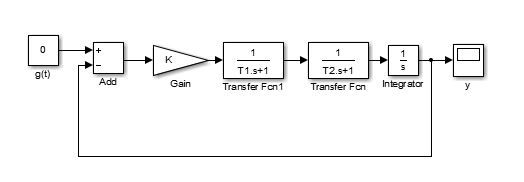
\includegraphics[width = 0.8\linewidth]{sxema} \\
   \centering Рисунок 1 - Схема моделирования
\end{figure}
\hfill\\*
\newpage
\section*{\centering 1 Устойчивость системы}
На рисунках 2, 3, 4 и 5 показаны преходные характеристики системы при различный $k$ и $T_2 = 0.1$. Соответственно на рисунке 2 при $k = 3$,на рисунке 3  при $k = 0$,на рисунке 4 при $k = 12$,на рисунке 5 при $k = 15$. \\
\begin{figure}[h]
	\centering
	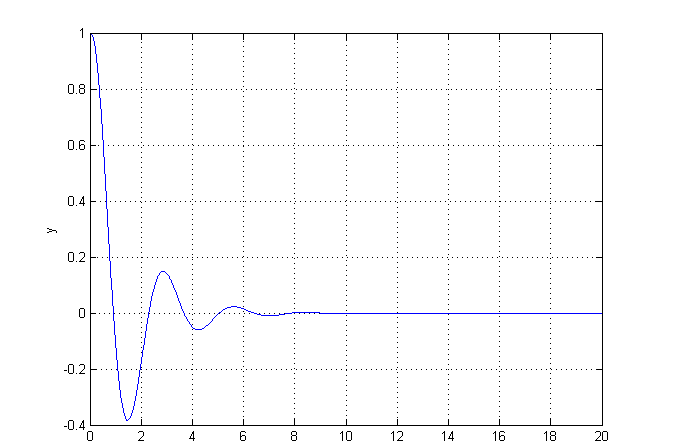
\includegraphics[width = 1\linewidth]{1.png} \\
  \centering Рисунок 2 - Устойчивая система при К=3
\end{figure} 
\hfill\\*
\newpage
\begin{figure}[h]
	\centering
	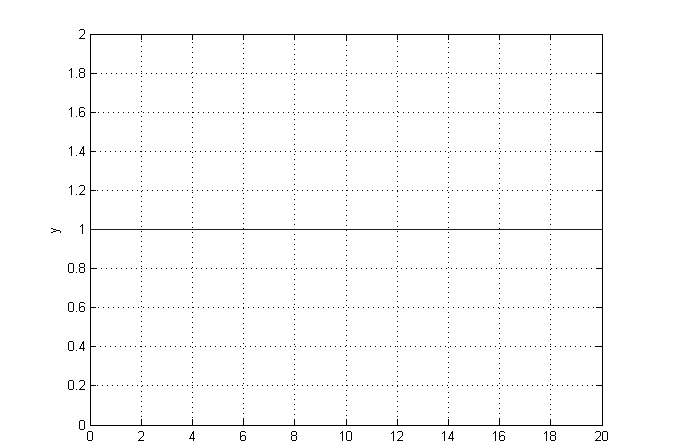
\includegraphics[width = 1\textwidth]{2.png} \\
  \centering Рисунок 3 - Граница устойчивости нейтрального типа при К=0
\end{figure}
\hfill\\* 
\begin{figure}[h!]
	\centering
	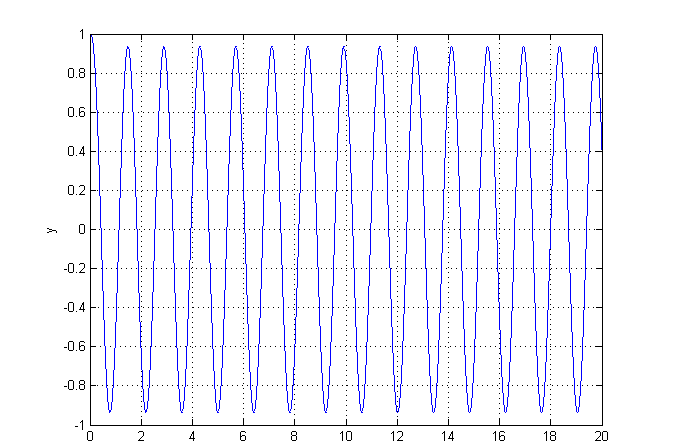
\includegraphics[width = 1\textwidth]{3.png} \\
  \centering Рисунок 4 - Граница устойчивости колебательного типа при К=12
\end{figure} 
\hfill\\*
\begin{figure}[h!]
	\centering
	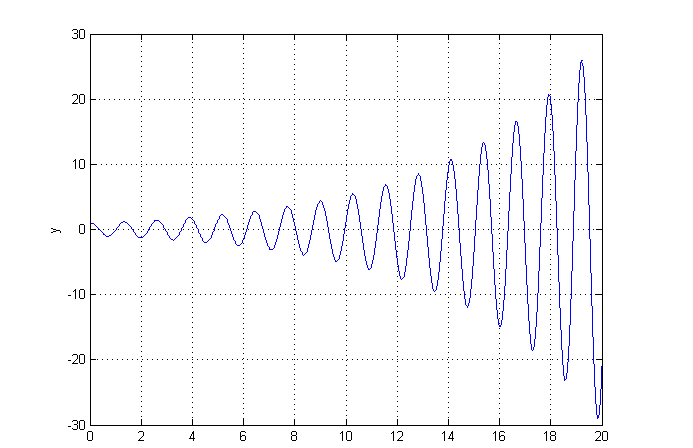
\includegraphics[width = 1\textwidth]{4.png} \\
  \centering Рисунок 5 - Неустойчивость системы при К=15
\end{figure} 
\hfill\\*
\newpage
\section*{\centering 2 Анализ устойчивости системы}

Предаточная функция исходной сисемы выглядит следющим образом:

\begin{equation}
W(s) = \frac{K}{T_1 T_2 s^3 + (T_1 + T_2)s^2 + s + K}
\end{equation}
\par Для анализа устойчивости системы составим матрицу Гурвица.

\begin{equation}
H_3 = \begin{bmatrix}
T_1 + T_2 &  K & 0 \\
T_1 T_2 & 1 & 0 \\
0 & T_1 + T_2 & 1
\end{bmatrix}
\end{equation}
\par Из этой матрицы можем, исользуя условие Гурвица, получить уравнение для системы на границы устойчивости колебательного типа.
\begin{equation}
\begin{cases}
T_1 + T_2 - K T_1 T_2 = 0 \\
T_1 + T_2 > 0 \\
K > 0
\end{cases}
\end{equation}
\begin{equation}
K =\frac{T_1 + T_2}{T_1T_2}
\end{equation}

\begin{table}[h]
		\caption{ Сравнительный анализ теоретического и экспериментального расчета границы устойчивости системы}
		
        \begin{center}
        
        
		\begin{tabular}{|p{0.05\linewidth}|p{0.05\linewidth}|p{0.05\linewidth}|p{0.05\linewidth}|p{0.05\linewidth}|p{0.05\linewidth}|p{0.05\linewidth}|p{0.05\linewidth}|p{0.05\linewidth}|p{0.05\linewidth}|p{0.05\linewidth}|}
			\hline
			\rule{0cm}{0.5cm}
			$T_2$,c & 0.1 & 0.5 & 1 & 1.5 & 2 & 2.5 & 3 & 4 & 4.5 & 5\tabularnewline	
			\cline{1-11}
			$K_e$ & 12.2 & 4.1 & 2.9 & 2.6 & 2.4 & 2.3 & 2.1 & 2 & 2 & 2\\
			\cline{1-11}
		    $K_p$ & 12 & 4 & 3 & 2.67 & 2.5 & 2.4 & 2.3 & 2.25 & 2.2 & 2.2\\
				\hline
			
		\end{tabular}
\end{center}
\end{table}

	Получив все необходимые уравнения мы можем построить график зависимости $K(T_2)$, $T_2 \in [0.1, 5]$. Как видно из уравнения (2) - эта зависимость является гиперболой, в случае же уравнения (3). График данной зависимости представлен ниже на рисунке 6 и 7. \\
	\hfill\\*


\begin{center}
\begin{tikzpicture}
\begin{axis} [
xlabel = {$T_2$, c},
grid = major,
height = 220,
width = 320,
ylabel = {$K_p$}
]

\addplot coordinates {
	( 0.1, 12 )
	( 0.5, 4 )
	( 1, 3 )
	(1.5, 2.67)
	( 2, 2.5 )
	( 2.5, 2.4)
	( 3, 2.3 )
	( 4, 2.25 )
	( 4.5,2.2 )
	( 5, 2.2 )};
\end{axis}
\end{tikzpicture}
\end{center}
\begin{center}
 \centering Рисунок 6 - Расчетная граница устойчивости
\end{center}
\begin{center}
\begin{tikzpicture}
\begin{axis} [
xlabel = {$T_2$, c},
grid = major,
height = 220,
width = 320,
ylabel = {$K_e$}
]

\addplot coordinates {
	( 0.1, 12.2 )
	( 0.5, 4.1 )
	( 1, 2.9 )
	(1.5, 2.6)
	( 2, 2.4 )
	( 2.5, 2.3)
	( 3, 2.1 )
	( 4, 2 )
	( 4.5,2 )
	( 5, 2 )};
\end{axis}
\end{tikzpicture}
\end{center} 
\begin{center}
 Рисунок 7- Эксперементальная  граница устойчивости 
\end{center}
\newpage
\section*{\centering Выводы}
При проектировании систем большое значение имеет определение областей устойчивости в плоскости реальных параметров, присущих системе.\par
 В данной работе, изменяя параметры $K$ и $T_2$, а $T_1$ оставляя неизменным , с помощью математического моделирования и аналитических методов мы построили границы устойчивости системы исходя из условия Гурвица.\par Данные полученные при математическом моделировании и аналитическом методе совпали. 

\end{document}
